\documentclass{article}
\usepackage{graphicx, amsmath}
\graphicspath{ {./images/} }


\title{Ch. 7.1-7.2 HW}
\author{Principles of Microeconomics}
\date{\today}

\begin{document}

\maketitle

\subsection*{Quick Quiz}

\begin{enumerate}

\item (b) --
	\begin{align*}
	CS_A &= 12 - 6 = 6 \\
	CS_B &= 8 - 6 = 2 \\
	CS_C &= 0 \\
	CS_{mkt} &= 6 + 2 = 8
	\end{align*}

\item (b) --
	\begin{align*}
	CS_A &= 12 - 3 = 9 \\
	CS_B &= 8 - 3 = 5 \\
	CS_C &= 4 - 3 = 1 \\
	CS_{mkt} &= 9 + 5 + 1 = 15 \\
	\Delta CS_{mkt} &= 15 - 8 = 7
	\end{align*}
	
\item (d) --

	\begin{center}
	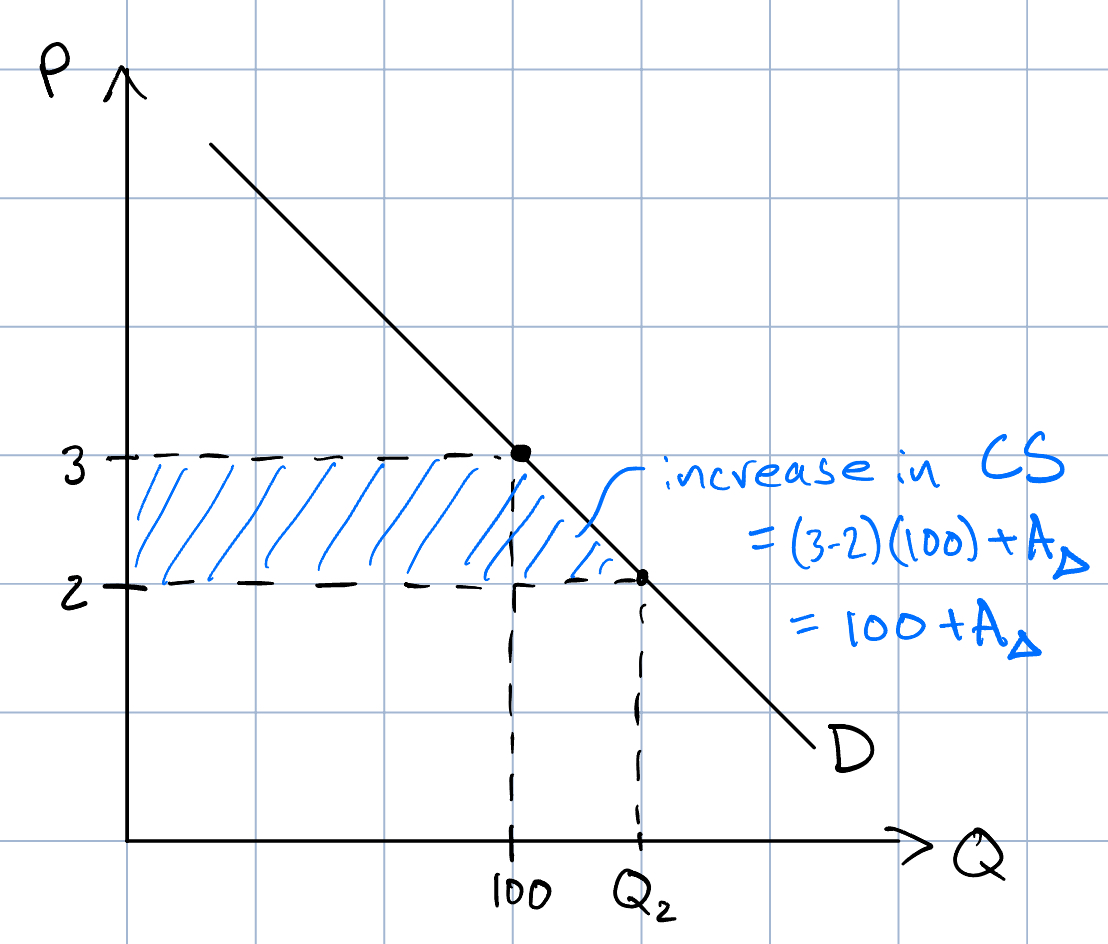
\includegraphics[width = 0.5\textwidth]{qq3}
	\end{center}
	
\end{enumerate}

\subsection*{Problems \& Applications}

\begin{enumerate}

\item 

	\begin{enumerate}
	
	\item

		\begin{align*}
		CS &= WTP - P \\
		240 &= WTP - 360 \\
		600 &= WTP
		\end{align*}
		
	\item
		
		\begin{align*}
		CS &= 600 - 270 \\
		CS &= 330
		\end{align*}
		
	\item She wouldn't have bought an iPhone because \$750 is more than her willingness to pay. With no purchase, her consumer surplus would have been 0.
		
	\end{enumerate}
	
\item The freeze reduces the supply of lemons, so the supply curve shifts left. That increases the price and decreases the quantity of lemons sold, so consumer surplus decreases.

	\begin{center}
	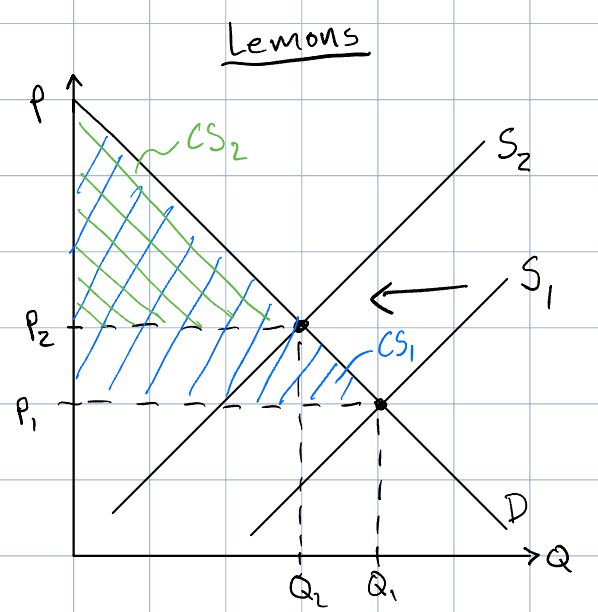
\includegraphics[width = 0.5\textwidth]{paa2_lemons}
	\end{center}
	
Lemons are an input to lemonade, so when the price of lemons increases, the supply of lemonade decreases. The supply curve for lemonade shifts left which increases the price and decreases the quantity of lemonade sold. As a result, consumer surplus goes down.

	\begin{center}
	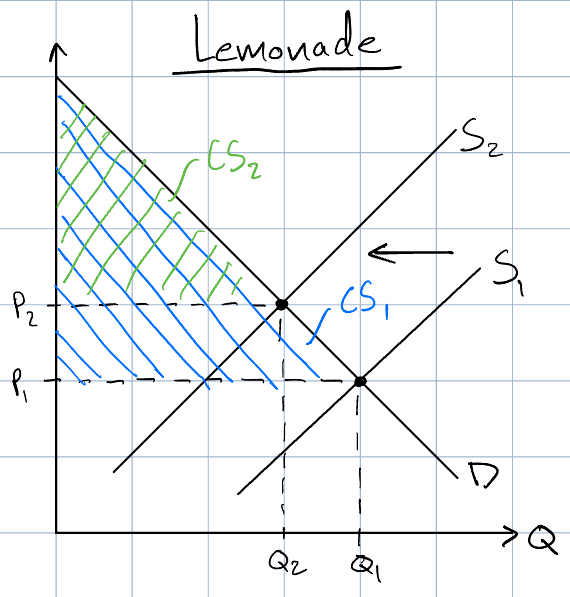
\includegraphics[width = 0.5\textwidth]{paa2_lemonade}
	\end{center}

\end{enumerate}

\end{document}